\documentclass{turabian-thesis}

\usepackage{graphicx}
\usepackage{subcaption}
\usepackage{pslatex}
\usepackage{amsthm}
\usepackage{amsmath}
\usepackage{amssymb}
\usepackage{mathtools}
\usepackage{bm}
\usepackage{paralist}
\usepackage[utf8]{inputenc}
\usepackage{multicol} 
\usepackage[hidelinks]{hyperref}
\usepackage{nameref}

\DeclareUnicodeCharacter{2215}{\textminus}
\usepackage{algorithm}
\usepackage{algpseudocode}
\algdef{SE}[DOWHILE]{Do}{DoWhile}{\algorithmicdo}[1]{\algorithmicwhile\ #1}%

\newtheorem{theorem}{Theorem}
\newtheorem{lemma}{Lemma}
\newtheorem{corollary}{Corollary}
\newtheorem{claim}{Claim}
\newtheorem{definition}{Definition}
\newtheorem{problem}{Problem}

\newcounter{case}[section]
\newenvironment{case}[1][]{\refstepcounter{case}\par\medskip
   \textbf{Case~\thecase. #1} \rmfamily}{\medskip}
   
\newcounter{subcase}[case]
\newenvironment{subcase}[1][]{\refstepcounter{subcase}\par\medskip
   \textbf{Case~\thecase.\thesubcase. #1} \rmfamily}{\medskip}

\begin{document}

\frontmatter
\thispagestyle{empty}

\begin{center}
   
   \textbf{Hybrid Model for Interpretable Time Series Analysis}
   
   \vspace*{\baselineskip} 
      
   A THESIS \\
   Presented to the Department of Computer Science and Computer Engineering \\
   California State University, Long Beach
   
   \vspace*{\baselineskip} 

   In Partial Fulfillment \\
   of the Requirements for the Degree \\
   Master of Science in Computer Science \\
   Option in Computer Science
   
   \vspace*{\baselineskip} 

   Committee Members: \\
   Ju Cheol Moon, Ph.D \\
   Roman Tankelevich, Ph.D \\
   Seok-Chul Kwon, Ph.D

   \vspace*{\baselineskip} 

   College Designee: \\
   Hamid Rahai, Ph.D.
   
   \vspace*{\baselineskip} 

   By Ruben Rosales \\
   May 2020
\end{center}

\pagebreak

\chapter*{Abstract}

% In this thesis, we study interpretable machine learning as applied to complex-valued time series data. Scientists have studied the use of several machine learning methods such as Convolutional Neural Networks, Recurrent Neural Networks, and Support Vector Machines for time series classification. These methods, however, fall short of allowing users to visualize patterns within their dataset.

% To address this issue, we propose an interpretable hybrid model that can be extended to any time series dataset. Our architecture is composed of two models, an ensemble method of classifiers that functions as a black-box method, and a white-box model that encodes time series as an image, attempts to classify them through a CNN, and outputs all images correctly classified in both black-box and white-box models.

In this thesis, we study interpretable machine learning as applied to complex-valued time-series data. Scientists have studied the use of several machine learning methods such as Convolutional Neural Networks, Recurrent Neural Networks, and Support Vector Machines for time series classification. These methods, however, fall short of allowing users to visualize patterns within their dataset.

To address this issue, we propose an interpretable hybrid model that can be extended to any time series dataset. In the majority of existing work in the field of interpretability, black-box models tend to outperform white-box models consistently. However, instead of relying purely on one method, we propose a collaboration between the two. This gives us the performance of a black-box while allowing us to visualize features of the majority of our dataset. 

To accomplish this, we created a framework composed of two models, an ensemble method of classifiers that functions as a black-box method, and a white-box model that encodes time series as images. The white-box model attempts to classify them through a neural network and outputs all images correctly classified in both black-box and white-box models.

\addcontentsline{toc}{chapter}{Abstract}
\chapter{Acknowledgments}

\tableofcontents
\listofillustrations

\mainmatter
\chapter{Introduction}
\label{chap:introduction}

As time series datasets become ever so popular the need for deep learning models becomes greater.
In our black-box model, we analyze deep learning models such as Convolutional Neural Networks which have become increasingly popular and widely used in the last decade but their complex nature makes it difficult for users to understand what is going on inside \cite{wang_hybrid_2019}. So, as black-box models get more popular and increase in complexity the need for an interpretable accessory is needed so we propose a hybrid model consisting of a black-box for classification and an interpretable white-box model which highlights characteristics of a time series for users to understand.

The goal of our work is not to find an alternative to black-box methods but to provide a way for users to have an understanding of what features are prevalent in their dataset.

% \section{The need for interpretable models in management problems}
% The growth of mobile devices and demand for wireless data has created a need for igh quality spectrum sensing and adaptation to improve spectral allocation and interference mitigation is an important route by which we may achieve this.  however have been constrained to relatively specialized solutions which lack the generality needed to deal with a complex and growing number emitter types, interference types and propagation environments.
% This is a significant challenge in the community as expert systems designed to perform well on specialized tasks often lack flexibility and can be expensive and tedious to develop analytically.

\section{Contributions}
We focus on creating deep learning architectures to classify our datasets as well as extending existing work to create our white-box model. Our final results show how robust our black-box method is as well as support for our white-box model.


\chapter{Data}

We analyzed our model on three radio signal datasets generated using Spatial Modulation. Spatial Modulation is a transmission technique that uses multiple antennas. It maps a block of information bits to two units, one is a symbol chosen from a constellation diagram, and the second one is a unique transmit antenna number that is chosen from a set of transmit antennas \cite{mesleh_spatial_2008}. The method in which transmit antennas send and receive radio waves can be described through polarization. Two popular basis polarizations are horizontal linear, H, and vertical linear, V. Our datasets contain data horizontally transmitted and vertically received (HV) and data vertically transmitted and vertically received.


The two properties HV and VV, are given to us in raw discrete format. Both properties consist of time and amplitude values but vary in length and in how they are processed. The raw signal consists of over 31,000 data points with the exact time it was received. The size of the discrete data can vary from 22 to 44 data points and is a processed representation of the raw signal that has equally spaced values. In this thesis we focus on discrete data given that it is closer to datasets in real-world situations.

% [ What is raw signal and discrete, compare them, ]
% [explain hv, vv]

\chapter{Related Work}
\label{chap:relatedwork}

\chapter{Preprocessing}
\label{chap:preprocessing}

Radio signal data is presented in a complex-valued format that is unusable in a typical neural network, so in an attempt to make our model robust and reduce any complexity, we focused on using real values as features.

We tried numerous methods to extract real-valued features, including Fourier Transform, Short Time Fourier Transform, a custom sliding window method, and polar coordinates taken directly from the signals amplitude/phase value. Before applying any of these methods, we normalized all data using L2 normalization.

% \section{What is it?}
% [what is feature extraction]

% % maybe?
% % Data pre-processing is concerned with the analysis and manipulation of the collected spectrum data to arrive at potentially good wireless data representations. The raw samples organized into data vectors rk in the previous block are pipelined as input for signal processing (SP) tools that analyze, process and transform the data to arrive at simple data representations such as frequency,
% % amplitude, phase and spectrum, or more complex features
% % xk such as e.g. cyclostationary features. In addition, feature
% % learning such as deep learning may be utilized to automatically
% % extract more low-level and high-level features. In many ML
% % applications the choice of features is just as important, if not
% % more important than the choice of the ML algorithm.



\section{Transformations}


\subsection{Fourier Transform}
% [Recall we can write a complex number in terms of its magnitude and phase
% (i.e., its polar representation). ]

% Transformation 1 : STFT/ FT
% [what is it]

% [fft formula]
The Fourier Transform (FT) is a mathematical tool that decomposes any function into a sum of sinusoidal basis functions. Each basis function is a complex value of a frequency, so it allows us to view our data in the frequency domain as opposed to amplitude.

One of the shortcomings of the FT is rooted in the Heisenberg Uncertainty Principle (HUP) \cite{hill_uncertainty_nodate}.  The HUP states that the position and velocity of an object cannot be simultaneously measured, which can be applied to the time-frequency information of a signal. This means we cannot know which spectral components exist at any given time. The closest we can get is sampling at different ranges of time and finding a range of frequencies within that time frame. This method is described as the Short-Time Fourier Transform.


% The Fourier Transform is a magical mathematical tool. The Fourier Transform decomposes any function into a sum of sinusoidal basis functions. Each of these basis functions is a complex exponential of a different frequency. The Fourier Transform, therefore gives us a unique way of viewing any function - as the sum of simple sinusoids.

% The Fourier Series showed us how to rewrite any periodic function into a sum of sinusoids. The Fourier Transform is the extension of this idea to non-periodic functions.

% While the Fourier Transform is a beautiful mathematical tool, its widespread popularity is due to its practical application in virtually every field of science and engineering. It's hard to understand why the Fourier Transform is so important. But I can assure you it enables the solution to difficult problems be made simpler (and also makes previously unsolved problems solvable). In addition, the Fourier Transform gives us a new method of viewing the world, which is fantastic for giving a more intuitive feel for our universe.


\subsection{Short-Time Fourier Transform}
% [stft]
The Short-Time Fourier transform (STFT) is a Fourier related transform used to determine the sinusoidal frequency and phase content of local sections of a signal as it changes over time. \cite{hill_uncertainty_nodate}
Computing STF requires the signal to be divided into segments of equal length and then have the FT applied to that segment. This allows us to view the Fourier spectrum at a more granular level, which could potentially reveal different patterns amongst signals of different classes.

One of the issues with this method is that we can create very narrow window sizes, which gives us a better understanding of the data with respect to time, but we lose understanding of the frequency domain. Additionally, selecting an appropriate window size for segmenting the signal can be an arduous task that would require fine-tuning as well as increasing the dimensionality of our dataset.

% The problem with STFT is the fact whose roots go back to what is known as the Heisenberg
% Uncertainty Principle. This principle originally applied to the momentum and location of
% moving particles, can be applied to time-frequency information of a signal. Simply, this principle
% states that one cannot know the exact time-frequency representation of a signal, i.e., one cannot
% know what spectral components exist at what instances of times. What one can know are the
% time intervals in which certain bands of frequencies exist, which is a resolution problem.
% The problem with the STFT has something to do with the width of the window function that is
% used. To be technically correct, this width of the window function is known as the support of
% the window. If the window function is narrow, then it is known as compactly supported. This
% terminology is more often used in the wavelet world, as we will see later.

% The problem is that when you are studying a real signal it would be useful to know what the ‘instantaneous frequency’ of the signal is. The instantaneous frequency is the exact frequency of a signal at an exact moment in time. For instance if I was listening to a music track I would like to be able to say ‘at 1 min 59.0423 seconds into the music track the so,und is 1563.2 Hz’. Unfortunately the Fourier Transform cannot do this because there exists a minimum amount of uncertainty between the frequency and time domains, like Heisenberg has a minimum amount of uncertainty between the speed and position of a particle (the area of the box). You can know the moment in time you want to find the frequency for (like the blue box), but because there is a minimum uncertainty, the box of has to stretch out across frequency, meaning that you are unsure of the frequency at that moment in time.

% The best you can do with a Fourier Transform is to sample a range of time (for instance, the time signal between 1 min 58 sec and 1 min 59 sec in a song) and find a range of frequencies that were played over that amount of time, as represented by the black box. An example of this can be seen by looking at the third picture in the post again. There is a signal over a range of time (e.g. someone saying ‘hello’) and the frequency graph is the range of frequencies recorded over that time.



% [purpose and motivation? Behind making it ang/abs]

% [definition plus method]



\subsection{Sliding Window Method}

We propose a method similar to STFT but to reduce the size of the data we take the mean at each window which would turn our size into size N where N is equal to the number of windows we use. This performed as well as STFT and gave us the advantage of reducing the dimensionality of our data. 

\subsection{Polar Coordinates}

% Transformation 2: Amplitude / Phase
The representation of a complex number as a sum of a real and imaginary number, z = x + iy, is called its Cartesian representation. For every cartesian point, we calculate its radius and angular distance which are real values and use those as features. This method outperformed the previous three methods but limited our feature size which made it difficult to get consistent accuracy across all three of our datasets.

\subsection{Wavelets}

Wavelets are similar to the FT in which they deconstruct a signal using representations of other signals. The key difference is that wavelet signals are finite in time and frequency as opposed to sin and cos signals, which can carry on forever \cite{strang_wavelets_1996}. This allows us to extract information from a signal with respect to time and location.


\begin{figure}[h!]
   \begin{center}
      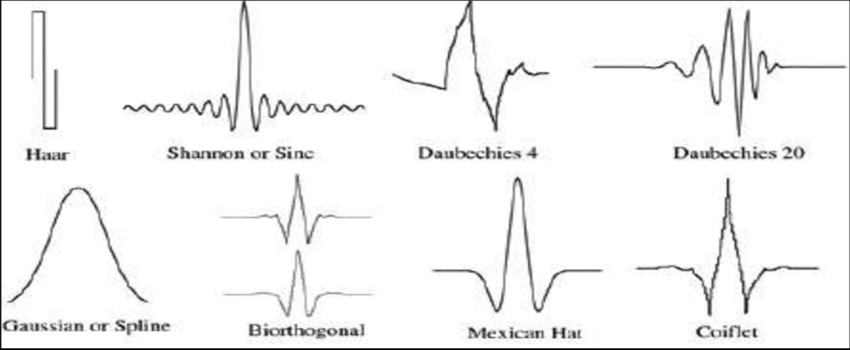
\includegraphics[scale=0.4]{../media/wavelet_families.png}
   \end{center}
   \caption{Example of different types of wavelets.}
   \label{fig:reinforcementAgent}
\end{figure}


The use of wavelets is called the wavelet transform, which is a technique in which a signal is analyzed using different versions of a dilated and translated basis functions called the mother wavelet. There are two types of wavelet transformations, discrete and continuous. In this thesis, we focus on discrete. Discrete Wavelet Transform uses a discrete set of wavelet scales and translations which decompose the signal into a mutually orthogonal set of wavelets. 

We take advantage of wavelets by applying discrete wavelet transforms as a filter-bank, which means it is composed of cascading high-pass and low-pass filters. This allows us to split a signal into several frequency sub-bands. We focus on wavelet decomposition as our feature extractor because it outperformed all other methods in terms of accuracy and training time.

% Transformation 3: Wavelets

% Wavelets are similar to the FT in which they deconstruct a signal using representations of other signals. The key difference is wavelet signals are finite in time and frequency as opposed to sin and cos signals which can carry on forever. Simply, this allows us to extract information from a signal which respect to time and location.

% The use of wavelets is called the wavelet transform which is a technique in which a signal is analyzed using different versions of a dilated and translated basis functionss called the mother wavelet. There are two types of wavelet transformations, discrete and continous. In this thesis we focus on discrete.

% DWT uses a discrete set of wavelet scales and translations which decompose the signal into mutually orthogional set of wavelets.

% One advantage of wavelets is they have varying window sizes so they can be wide for slow frequencies and narrow for faster ones this is handled by the property called scale [add figure].

% wavelets 


% Some properties of wavelets are orthogonality, zero mean, and are efficient at representing localized data and functions.



% Db4 wavelet http://wavelets.pybytes.com/wavelet/db4/

% Model 1:
% Model 2: 
% Model 3: 



% In the preprocessing stage we tried numerous combinations of features but found the best performing features to come from wavelet decomposition.




% Wavelets

% We take advantage of wavelets by applying discrete wavelet transforms as a filter-bank which means it’s composed of cascading high-pass and low-pass filters. This gives us the advantage of splitting a signal into several frequency sub-bands. Wavelet decompositions give us the advantage of gaining features that take into account frequency and time domains. 

% [explain why they performed better]


% [alternatives]


\section{Data Shape}
% [Shape of data comparison]

A neural network requires all data to be the same shape. However, because we downsample in wavelet decomposition, each data size is halved until making it impossible to place all levels of decomposition into the same dataset. In order to circumvent this, we tried two different methods, resampling the data and treating each level of decomposition as its own dataset.


\subsection{Resampling}

We use spline interpolation in order to resize each level of decomposition into a single array. We tested different sizes of interpolation from N to N/3, where N is the size of the largest discrete signal size, and found no reduction in performance.

\subsection{Each level}
Figure \ref{fig:multimodal_overview} depicts our model in which each level of decomposition is treated as its own dataset. We found no difference in accuracy compared to the resampling method. However, given that related work we found treated each decomposition level as its own dataset, we decided to go with this method. 


\chapter{Models}
\label{chap:models}

% [introduce models definitions]
% [EXPLAIN LOSS AND HOW ACCURACY IS MEASURED]


\section{Definition}
Machine learning algorithms can be seen as learning a target function (f) that maps input data (X) to an output (Y). There are several techniques to make this work, but we focus on nonparametric algorithms, namely Convolutional Neural Networks (CNN) and Long Short Term Memory networks (LSTM). Nonparametric algorithms are algorithms that attempt to make minimal assumptions about the form of the function so they can learn any form from data provided to it. An example would be a neural network because it has no prior knowledge about what it is classifying and attempts to generalize any new data points that it has not seen before.

\subsection{CNN}
% [cnn]

A Convolutional Neural Network is a type of deep neural network that can be applied to different domains such as computer vision or time series analysis. It consists of an input and output layer as well as hidden layers. A convolution is an operation between a vector of weights w against an input x. It consists of taking the dot product between m and x were in steps of a filter size defined by n.

Convolutional Neural Networks perform feature learning via non-linear transformations implemented as a series of layers. The input data is a multidimensional array, called a tensor. The input data is passed through an input layer, followed by a series of hidden layers to extract features, and finally, an output layer, which in the case of classification, gives a probability for each class. 

% create your own design
\begin{figure}[h!]
   \begin{center}
      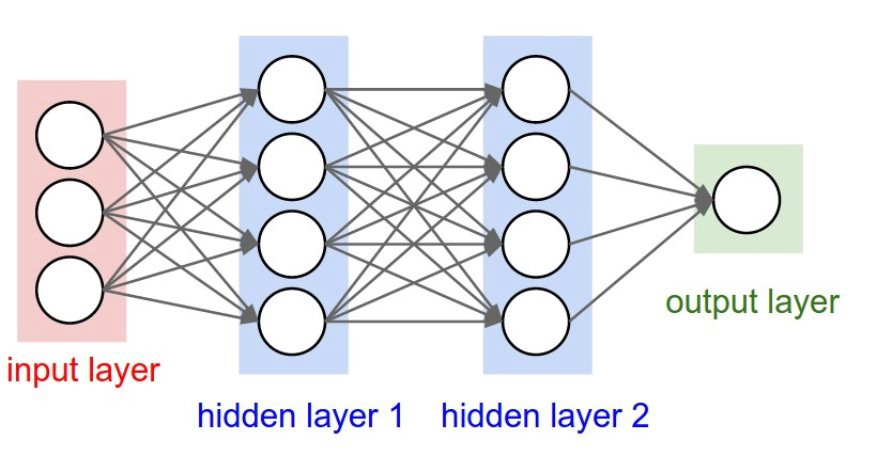
\includegraphics[scale=0.3]{../media/nn_highlight.jpeg}
   \end{center}
   \caption{Example of a Convolutional Neural Network.}
   \label{fig:reinforcementAgent}
\end{figure}

Hidden layers are crucial to neural networks because it is how a model can determine which data representations are useful for explaining the relationships in the given data. Each layer consists of several kernels that perform a convolution over the input; therefore, they referred to as convolutional layers. Kernels are feature detectors that convolve over the input and produce a transformed version of the data at the output. 




\subsection{LSTM}

% [lstm]
Long short-term memory (LSTM) is an artificial recurrent neural network (RNN) architecture used in the field of deep learning. Unlike standard feedforward neural networks, LSTM has feedback connections. It can process not only single data points but also entire sequences of data. 

A standard LSTM unit is composed of a cell, an input gate, an output gate, and a forget gate. The cell remembers values over arbitrary time intervals, and the three gates regulate the flow of information into and out of the cell.

LSTM networks are well-suited to classifying, processing, and making predictions based on time series data since there can be lags of unknown duration between significant events in a time series. LSTMs were developed to deal with the exploding and vanishing gradient problems that can be encountered when training traditional RNNs. 

\begin{figure}[h!]
   \begin{center}
      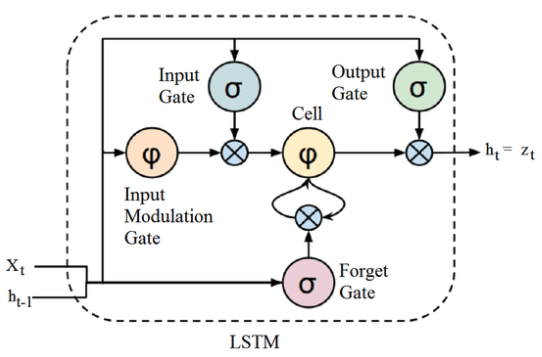
\includegraphics[scale=0.5]{../media/lstm_highlight.png}
   \end{center}
   \caption{Example of a LSTM unit.}
   \label{fig:reinforcementAgent}
\end{figure}

\subsection{Multimodal Deep Learning}

% [multimodal]
Due to the superior performance and computationally tractable representation capability in multiple domains such as visual, audio, and text, deep neural networks have gained tremendous popularity in multimodal learning tasks \cite{kim_multimodal_2018}. Typically, domain-specific neural networks are used on different modalities to generate their representations, and the individual representations are merged or aggregated. Finally, the prediction is made on top of aggregated representation, usually with another neural network to capture the interactions between modalities and learn complex function mapping between input and output.


% [explain architectures]

\section{Architectures Used}

\subsection{CNN}

Our CNN architecture consists of 3 convolutional layers each followed by a batch normalization and dropout layer then finally connected to two dense layers (Figure X). We attempted to make it deeper but found inconsistent performance across all of our datasets.
% [add figure]

\begin{figure}[h!]
   \begin{center}
      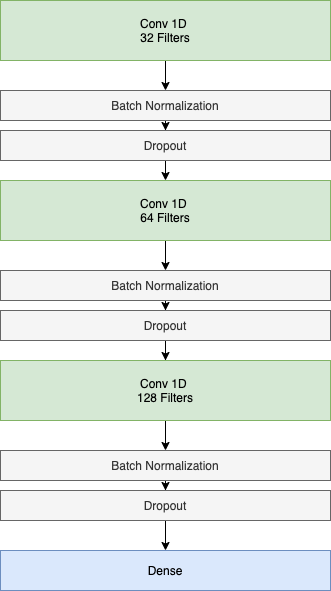
\includegraphics[scale=0.6]{../media/cnn_model.png}
   \end{center}
   \caption{CNN architecture used in our black-box model.}  
    \label{fig:cnn_model}
\end{figure}

\subsection{LSTM}
We wanted to keep our LSTM network as small as possible, for X purposes, so we went with two LSTM layers of 128 hidden states and a dropout rate of 4/10  followed by a dense layer of 128 connections. We attempted different state sizes but found 128 to be the smallest number with the best consistent performance.

% [add figure]
\begin{figure}[h!]
   \begin{center}
      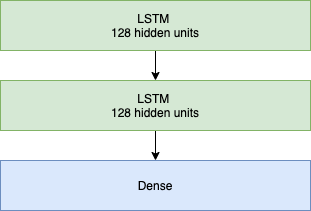
\includegraphics[scale=0.6]{../media/lstm_model.png}
   \end{center}
   \caption{LSTM architecture used in our black-box model.}
   \label{fig:lstm_model}
\end{figure}


\subsection{Final Model}

We propose a multimodal learning architecture for the purpose of time series classification which is illustrated in Figure \ref{fig:multimodal_overview}. The multimodal architecture allows our data to vary in size and given that all three levels of decomposition have varying length due to downsampling, we propose each model to learn the representation of each distinct feature. For this architecture we propose two architectures, a 1D CNN and an LSTM, in which we employ two CNN’s and 1 LSTM. They are all concatenated after their respective dense layer after which they perform classication via a softmax layer. 
% [add figure]

\begin{figure}[h!]
   \begin{center}
      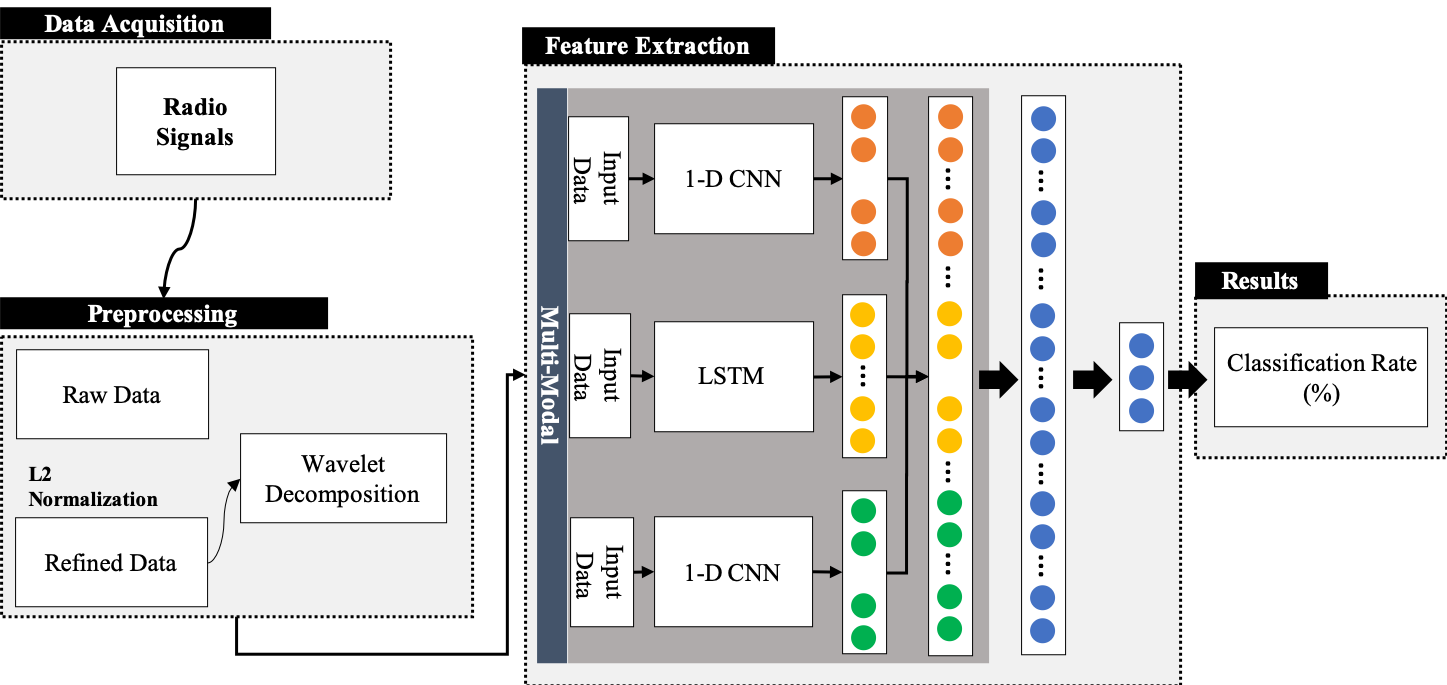
\includegraphics[scale=0.6]{../media/multimodal_overview.png}
   \end{center}
   \caption{Overview of our black-box model.}
   \label{fig:multimodal_overview}
\end{figure}


% \section{mtf}

% We approach our MTF is slightly different than  because instead of performing it over all samples in the dataset we perform it for every signal. 

% The three attributes we use are values are the absolute value of HV SBR, the absolute value of VV SBR, and a mathematical combination of the two (Figure X).

% [add figure]

 
\chapter{Markov Transition Fields}
\label{chap:mtf}

% We propose a framework similar to [] for encoding dynamical transition statistics,
% but we continue their work by considering ith order Markov transition probabilities.
% Given a time series X, we decompose its magnitude axis into two separate
% properties by representing it as a polar coordinate, Xangular and Xradial. We then
% identify the Q quantile bins for both properties and the temporal values Xtime
% and assign each x in Xangular, Xradial, Xtime to its corresponding bin qj (j in
% [1, Q]). Thus we construct three QxQ adjacency transition matrices, Wangular,
% Wradial, Wtime, by counting transitions among quantile bins in the manner of a
% ith order Markov chain along the time axis.

% W does not take into account the temporal axis so to prevent any information
% loss we construct a Markov Transition Field (MTF) for each W. The MTF
% denotes the probability of transitioning from qi to qj for each x in X. This,
% in turn, allows us to consider the transition probability on the magnitude and
% temporal axis.

% As described in [] the MTF encodes the multi-span transition probabilities
% of the time series, but given that we have three different M’s we modify their
% approach and consider each M to be a separate color channel of RGB where
% Mangular is red, Mtime is blue, Mradial is green. 

% \section{Markov Transition Field}

We propose a framework similar to \cite{wang_encoding_nodate}  for encoding dynamical transition statistics, but we continue their work by i\textsuperscript{th} order Markov transition probabilities.

Given a time series X, we decompose its magnitude axis into three separate properties, P\textsubscript{1},  P\textsubscript{2},  P\textsubscript{3}. We then identify the Q quantile bins for each property  and assign each $x \in P\textsubscript{1},  P\textsubscript{2},  P\textsubscript{3}$ to its corresponding bin q\textsubscript{j} (j in [1, Q]). Thus, we construct three QxQ adjacency transition matrices, W\textsubscript{1}, W\textsubscript{2}, W\textsubscript{3}, by counting transitions among quantile bins in the manner of a i\textsuperscript{th} order Markov chain along the time axis.

\begin{figure}[h!]
   \begin{center}
      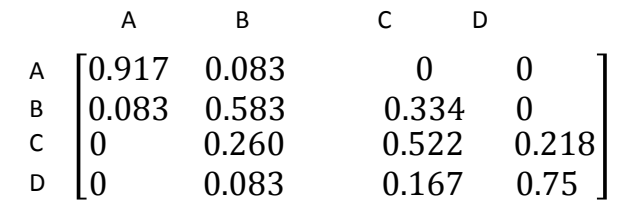
\includegraphics[scale=0.6]{../media/mtf_q.png}
   \end{center}
   \caption{Example of QxQ quantile bin matrix used to calculate MTF.}
   \label{fig:mtf_q}
\end{figure}
 

%summation %. This effectively removes any sensitivity to the X’s distribution and temporal dependency to each time step t i. To account for any information loss after removing the temporal dependency, we follow the same approach as \cite{wang} and construct a Markov Transition Field for each property like so: %some figure%




W does not take into account the temporal axis so to prevent any information loss we construct a Markov Transition Field, M, for each W. The MTF denotes the probability of transitioning from q\textsubscript{i} to q\textsubscript{j} for each $x \in P$. This, in turn, allows us to consider the transition probability on the magnitude and temporal axis.

\begin{figure}[h]
  \centering
  M =
  \[\begin{bmatrix}

  \text{W\textsubscript{ij}} | \text{$x\textsubscript{1} \in q\textsubscript{i}$, $x_{1} \in q\textsubscript{j}$}
  & \dots &
  
  \text{W\textsubscript{ij}}  |  \text{$x_{1} \in q\textsubscript{i}$, $x_{n} \in q\textsubscript{j}$} 
  
  \\
  
  \vdots &  \ddots & \\
  
  \text{W\textsubscript{ij}} | \text{$x_{n} \in q\textsubscript{i}$, $x_{1} \in q\textsubscript{j}$}
  & \dots &
  \text{W\textsubscript{ij}} | \text{$x_{n} \in q\textsubscript{i}$, $x_{n} \in q\textsubscript{j}$} \\
  
  
  \end{bmatrix}\]
  \caption{Markov Transition Field where  W\textsubscript{ij} denotes the transition probability from quantile i to j.}
  \label{fig:mtf}
\end{figure}

As described in \cite{wang_encoding_nodate} the MTF encodes the multi-span transition probabilities of the time series, but given that we have three different M's we modify their approach and consider each M to be a separate color channel of RGB where M\textsubscript{1} is red, M\textsubscript{2} is blue, M\textsubscript{3} is green. Since each row in M is a probability from 0 to 1 we multiply it by 255 to get a color value.

\chapter{Main Results}
\label{chap:results}

\section{Black-Box Model}
Our black-box model is constructed of three different architectures, 1 LSTM and 2 CNN’s, that are concatenated at the dense layer. The three features we use are amplitude/phase of each level of decomposition for HV and VV. We chose four because we wanted to take into consideration both HV / VV in the event that one had more descriptive features than the other.

To test our model we split our data into training and test sets by randomly selecting 70\% of our data as test and left the other 30\% as our test set. We then performed 3 fold cross validation and took the average of our results as our final outcome.

\begin{figure}[h!]
   \begin{center}
      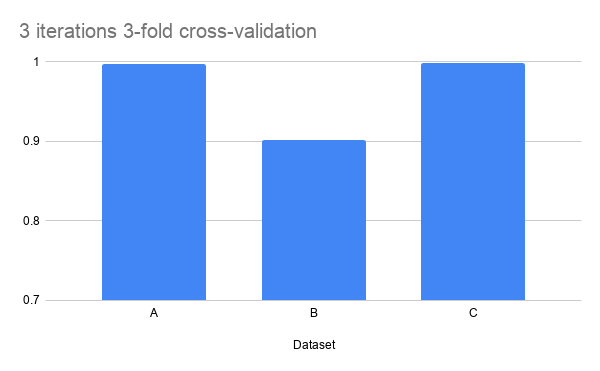
\includegraphics[scale=0.6]{../media/results.png}
   \end{center}
   \caption{Results}
   \label{fig:final_results}
\end{figure}


\section{Dataset B}

Given that this dataset is ten times larget than our other two datasets we wanted to try different training and test splits, namely we went as low as 8\% for training data and used the remaining 92\% as test data. We ran the same number of cross validation as our previous tests and found minimal difference in performance.


% [add table for results]

\section{White-Box Model}
Our white box is composed of a model that takes in raw data as an input and converts each signal into an image through the MTF method. We then pass those images through a CNN and those that are correctly classified are shown to the user.

In order to classify those images we created a CNN for it specifically and avoided using our existing CNN in order to make it deeper and increase performance when images aren’t that classifiable. We explored several architectures, such as, ResNet, Inception-v4, and AlexNet but we decided to create an architecture similar to AlexNet due to the variation and size of datasets we used we couldn’t create a model deeper or more complex than it otherwise performance would drop because we didn’t have enough data to properly train it.


\begin{figure}[h!]
   \begin{center}
      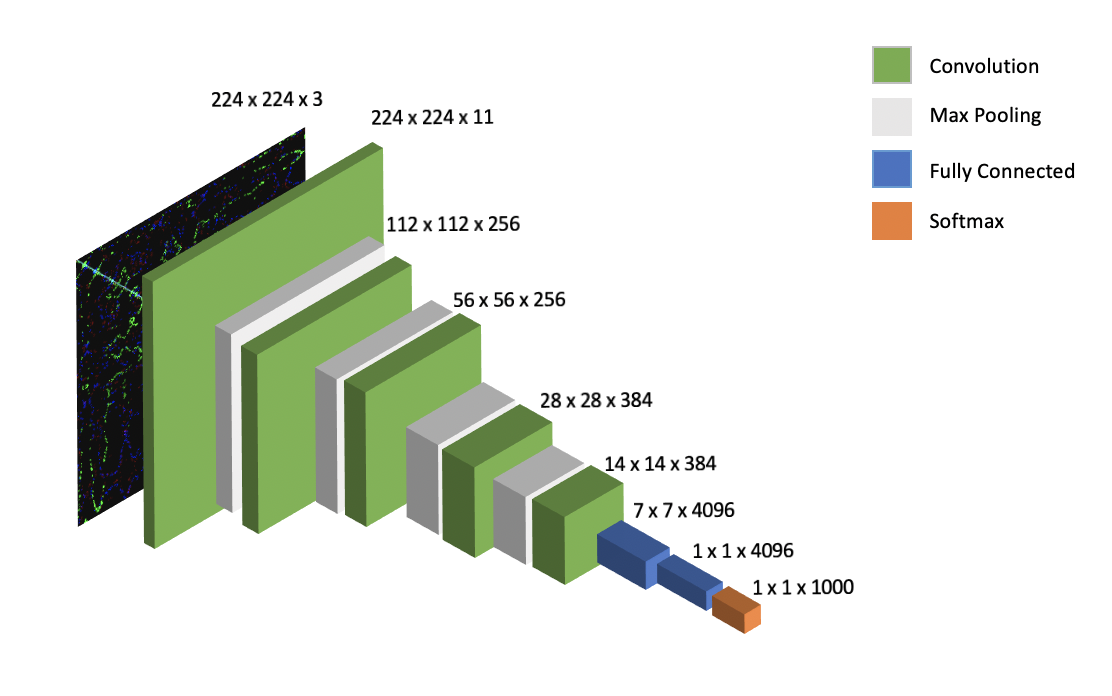
\includegraphics[scale=.7]{../media/2d_cnn.png}
   \end{center}
   \caption{CNN architecture for classifying images generated through MTF's.}
   \label{fig:mtf_cnn_results}
\end{figure}

% [add results]


\chapter{Conclusion}
\label{chap:conclusion}
Throughout this thesis, we have stressed the importance of a hybrid machine learning algorithm as well as providing a framework that can successfully classify and visualize different classes when applied to time-series data. 

We proposed an extension to existing work described in [] so users can visualize their data while being able to classify them with 60\% accuracy on our dataset and model. We also created a robust black-box model consisting of two different deep learning architectures that consistently provided competitive accuracy.

In the future, we would like to explore other methods for our white-box model that would act as an alternative to Markov Transition Fields in hopes that it produces higher accuracy than our current model. Additionally, we would like to extensively test our model on different time-series datasets, not just radio signal datasets.


\bibliography{../references/main}
\bibliographystyle{plain} 

\end{document}
